
%PREAMBLE
%%%%%%%%%%%%%%%%%%%%%%%%%%%%%%%%%%%%%%%%%%%%%%%%%%%%%%%

\documentclass[titlepage,norsk]{article}
\usepackage{babel,graphicx}
\usepackage[utf8]{inputenc}
\title{Geokomai}
\author{ Sania Ahktar \and Øystein Heimark \and Eirik Hjelle
		\and Steffen Phøner Henriksen \and Odd Andreas Sørsæther \and Andreas Hagen}

%%%%%%%%%%%%%%%%%%%%%%%%%%%%%%%%%%%%%%%%%%%%%%%%%%%%%%%

\begin{document}
\maketitle


\section{Summary}


Vårt prosjektforslag går ut på å undersøke hvilken funksjonalitet som bør inngå i en vegapp. Denne vegappen er for billister og målet er å samordne informasjon fra mange forskjellige kilder. 
Beskrivelse

Det finnes per i dag forskjellige dataverktøy som gir brukere informasjon om vegforhold, men det er lite integrering mellom disse. De fleste fokuserer på en enkelt datakilde.

Vegappen skal være til hjelp for billisten og vise nyttig informasjon. Denne informasjonen kan være for eksempel værdata, trafikkmeldinger, trafikkuhell, trafikktetthet, ras, sanntidsinformasjon for fergeavganger. Målet er å koordinere informasjon fra flere forskjellige kilder, og prosjektet vil ta for seg hvilke kilder som er mest relevante. Noen eksempler kan være NVDB, Vegvesenet, yr.no, Direktoratet for naturforvaltning og NVE. 

Når data er samlet kan det brukes til å gi bruker en risikoprofil for den vegstrekningen de befinner seg på i sanntid. Det må presiseres at prosjektet går ut på å undersøke mulighetene som ligger i en applikasjon for billister. Utvikling av en prototype er krevende, og det må vurderes fortløpende om det er tid til dette innen rammene som gis. Sluttresultatet vil være en rapport. 

\newpage
%\tableofcontents

\section{Lorem Ipsum}

\footnote{Slik ser en fotnote ut}

\subsection{Neque porro quisquam est qui dolorem ipsum quia dolor sit amet, consectetur, adipisci velit..."}

\paragraph{Lorem ipsum dolor sit amet, consectetur adipiscing elit. Sed fermentum interdum pulvinar. Fusce ullamcorper arcu vitae metus ornare hendrerit. Praesent elit lorem, ultrices luctus vestibulum et, blandit id ligula. Class aptent taciti sociosqu ad litora torquent per conubia nostra, per inceptos himenaeos. Proin lorem leo, congue sit amet pharetra vitae, feugiat vitae dui. Curabitur nec purus ante.
Phasellus velit elit, sodales nec dignissim ac, laoreet ac leo. Aenean ut dolor nec eros vestibulum malesuada. Aenean placerat magna id leo iaculis id eleifend metus pharetra. Maecenas sed augue purus. Suspendisse pulvinar tortor quis nulla aliquet ac feugiat augue ultricies. Etiam in magna vitae risus ullamcorper aliquam. Duis ligula mauris, iaculis sed rutrum quis, sollicitudin eget lectus. Maecenas auctor mauris nec odio interdum sodales. Sed convallis, leo id dignissim faucibus, est neque accumsan lacus, ac fringilla nisi ligula ac risus.
}

\marginpar{Hvis dere vil skrive noe i margen ser det slik ut}

\subparagraph{Nunc aliquet neque turpis. Aliquam nec accumsan erat. Nam imperdiet, nulla sed elementum imperdiet, arcu neque lacinia dolor, non semper metus felis ac magna. Cum sociis natoque penatibus et magnis dis parturient montes, nascetur ridiculus mus. Praesent tristique augue ac urna vulputate ornare. Phasellus diam dui, mollis nec accumsan vitae, tempus sed nunc. Mauris fringilla, neque ut euismod consectetur, mi arcu ornare dui, a lacinia turpis tellus a orci. Nullam bibendum porta tellus, ut pellentesque lectus sodales id. Duis erat ante, dapibus vitae adipiscing et, iaculis at risus. Duis quis ante arcu, hendrerit volutpat tortor. Maecenas varius nibh facilisis ligula hendrerit tempor.
}

\begin{figure}[p]
\centering
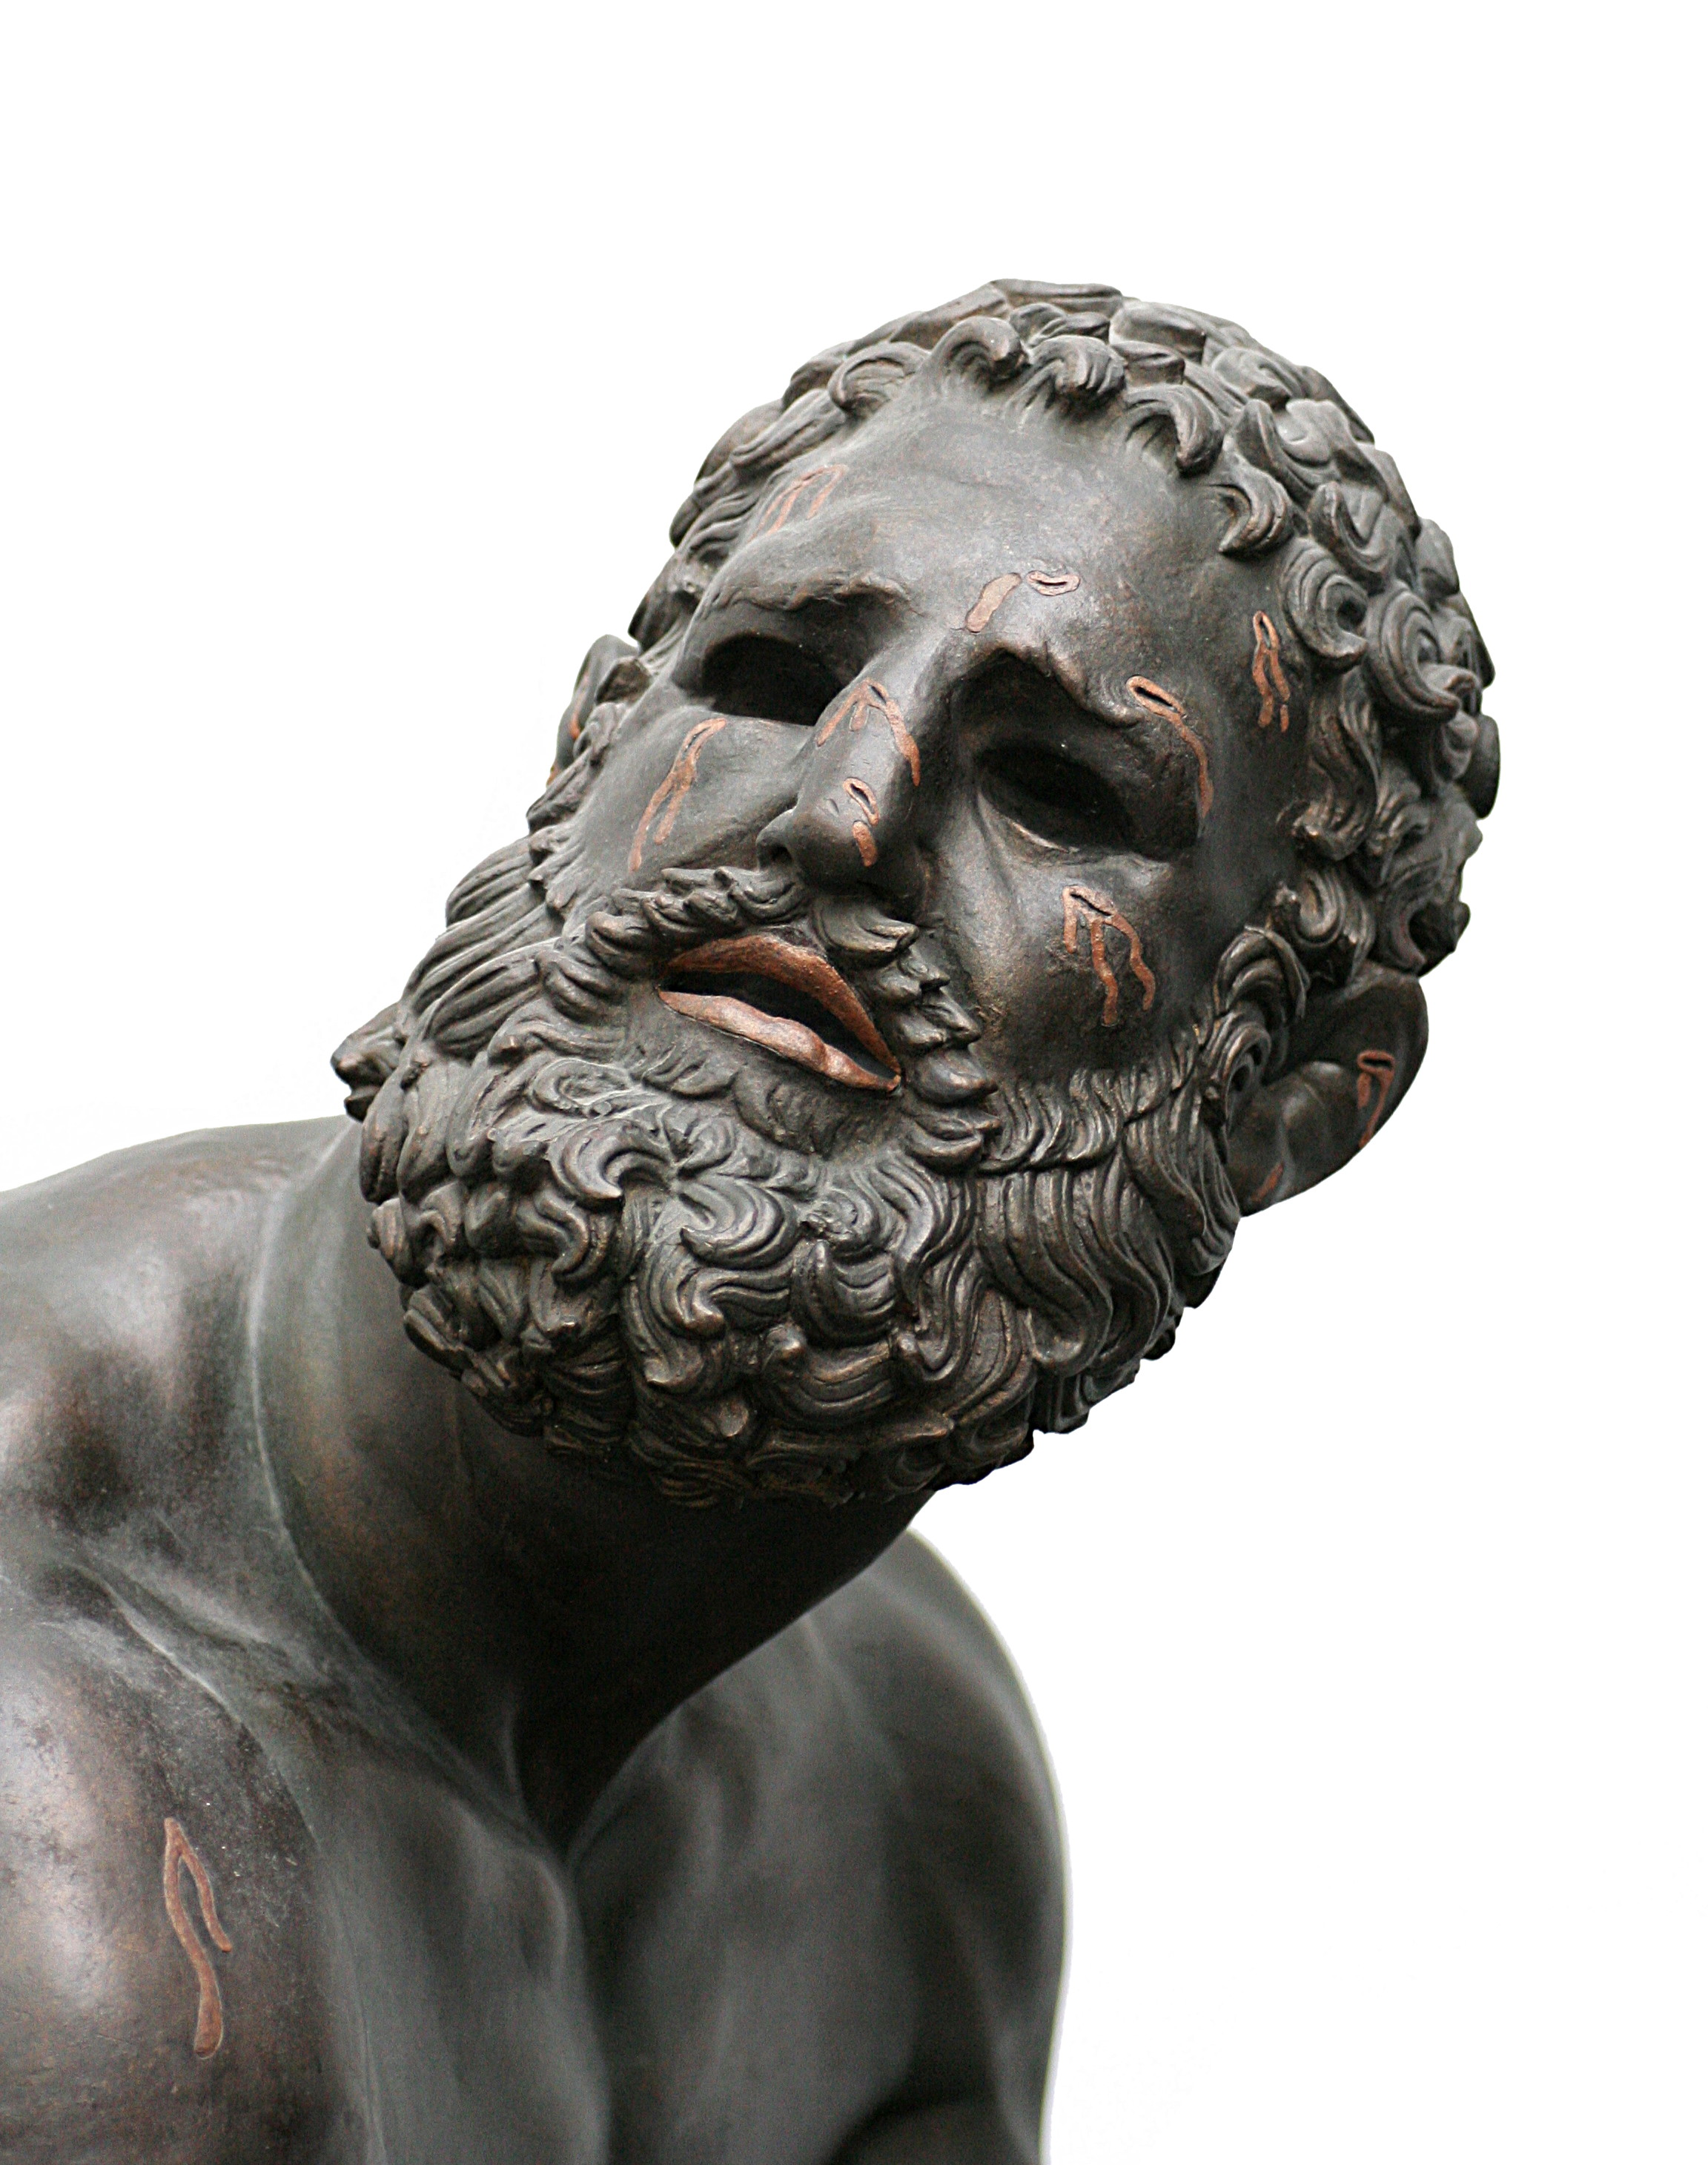
\includegraphics[scale=0.10]{pic.jpg}
\caption{Her setter du inn bildetekst}
\label{fig:awesome_image}
\end{figure}


\subparagraph{
Duis tristique arcu dictum massa gravida tempus. Sed sit amet ipsum leo, quis suscipit dolor. Mauris ornare, dolor a scelerisque imperdiet, nunc libero cursus felis, at vestibulum mauris urna nec tortor. Class aptent taciti sociosqu ad litora torquent per conubia nostra, per inceptos himenaeos. Vestibulum ante ipsum primis in faucibus orci luctus et ultrices posuere cubilia Curae; Fusce auctor commodo quam at mollis. Donec ut lacus aliquet nisl ullamcorper venenatis. Praesent convallis neque at urna dignissim ut hendrerit ante lacinia. Donec fermentum sapien at mi congue vel convallis enim posuere. Praesent tincidunt ipsum vitae lectus fringilla cursus. Proin dictum gravida interdum. Pellentesque vehicula ultrices iaculis. Nulla volutpat enim at mi euismod ac interdum ipsum gravida. Maecenas est velit, congue id ultricies at, auctor quis neque. Quisque viverra, augue in lobortis tincidunt, nibh tortor porttitor erat, id egestas libero ante posuere ante. Phasellus vel pharetra eros.
}

\appendices


\end{document}